\documentclass[a4paper, 11pt]{article}
\usepackage[utf8]{inputenc}
\usepackage[T1]{fontenc}
\usepackage{lmodern}
\usepackage{titlesec}
\usepackage{amsfonts}
\usepackage{amsmath}
\usepackage{color}
\usepackage[txtcentered=true, height=40pt, width=70pt]{thumbs}
\usepackage[left=1.5cm, top=2cm, right=2.5cm]{geometry}
\usepackage{subcaption}
\usepackage{circuitikz}
\usepackage{trfsigns}
\usepackage{pgfplots}
\usepackage{textcomp}
\usepackage{multicol}
\usepackage{upgreek}
\usepackage{empheq}
\usepackage{array}
\usepackage{float}

\pagenumbering{arabic}

\newcommand{\fancythumb}[2]{
	\addthumb{#1}{\large\sffamily\textbf{\space\space#1\vspace{5pt}}}{white}{#2}
}

\newcommand{\fancyformula}[2]{
        \small
        \raggedright{\sffamily\textbf{#1}}
        #2
}

\newcommand{\ftransform}{~~\laplace~~}

\usetikzlibrary{positioning}
\usetikzlibrary{calc}

\usepgfplotslibrary{fillbetween}
\pgfplotsset{compat=1.15}

\DeclareMathOperator{\Si}{Si}
\DeclareMathOperator{\sinc}{sinc}
\DeclareMathOperator{\sgn}{sgn}
\DeclareMathOperator{\rect}{rect}
\DeclareMathOperator{\ld}{ld}
\let\Re\relax
\let\Im\relax
\DeclareMathOperator{\Re}{Re}
\DeclareMathOperator{\Im}{Im}

\titleformat*{\section}{\sffamily\Large\bfseries}
\titleformat*{\subsection}{\sffamily\large\bfseries}
\titleformat*{\subsubsection}{\sffamily\normalsize\bfseries}
\titleformat*{\paragraph}{\sffamily\normalsize\bfseries}

\begin{document}

\section*{Abstastung und Quantisierung}
\begin{multicols}{2}
	\fancyformula{Abtasttheorem}{
		\[
			f_s \geq 2 ~ f_{\mathrm{max}} = f_{s, N}
		\]
	}

	\fancyformula{Nyquist-Frequenz}{
		\[
			f_N = \frac{1}{2} ~ f_s
		\]
	}

	\fancyformula{Nyquist-Rate}{
		\[
			f_{s, N} = 2 ~ f_{\mathrm{max}}
		\]
	}

	\fancyformula{Abtastung im Frequenzbereich}{
		Für $x_k = x(t + k / f_s)$
		\[
			X_\mathrm{sampled}(f) = f_s ~ \sum_{n = -\infty}^\infty X(f - n f_s)
		\]
	}

	\fancyformula{Grenzfrequenz Rekonstruktions-Tiefpass-Filter (RLP)}{
		\[
			f_\mathrm{max} < f_\mathrm{RLP} < f_s - f_\mathrm{max}
		\]
	}
\end{multicols}

\section*{Erstes Nyquist-Kriterium}
Bei der Schrittgeschwindigkeit $R_s = \frac{1}{T_s}$ erfüllt ein Impuls $g(t)$ das erste Nyquist-Kriterium, wenn
\[
	g(t) \overset{!}{=} \begin{cases}
		1 & t = 0\\
		0 & t = k ~ T_s, ~ k \neq 0, ~ k \in \mathbb Z
	\end{cases} \qquad \text{(Zeitbereich)}
\]
\[
	\Leftrightarrow
\]
\[
	\frac{\omega_s}{2 \pi} ~ \sum_{k = -\infty}^\infty G(\omega - k \omega_s) \overset{!}{=} 1 \quad \text{mit} ~ \omega_s = \frac{2 \pi}{T_s} \qquad \text{(Frequenzbereich)}
\]

Frequenzbereich intuitiv: Um $\ldots, ~ -\omega_s, ~ 0, ~ \omega_s, ~ 2 \omega_s, ~ \ldots$ verschobene Spektra addieren sich zu $1$ auf!
Wenn das erste Nyquist-Kriterium erfüllt ist, dann gibt es keine Intersymbol-Interferenz (ISI).

\textbf{Hinweis:} Das zweite Nyquist-Kriterium ist heute kaum noch praxisrelevant.

\section*{Raised-Cosine-Impulsformung}
$\alpha$ \ldots ``roll-off''-Faktor, $T = \frac{1}{R_s}$ mit $R_s$ \ldots Symbolrate. Für $\alpha = 0$ ist der Raised-Cosine-Impuls ein $\sinc$-Impuls, d.h. ein idealer Tiefpass.

\begin{figure}[H]
	\begin{subfigure}{0.7\textwidth}
		\fancyformula{Spektrum $G(f)$}{
			\[
				G(f) = \begin{cases}
					1 & |f| \leq \frac{1 - \alpha}{2T} \\ \\
					\frac{1}{2} ~ \left(1 + \cos \left(\frac{\pi T}{\alpha} ~ (|f| - \frac{1 - \alpha}{2 T}) \right) \right) & \frac{1 - \alpha}{2 T} \leq |f| \leq \frac{1 + \alpha}{2 T} \\ \\
					0 & \text{sonst}
				\end{cases}
			\]
		}

		\fancyformula{Impulsantwort $g(t)$}{
			\[
				g(t) ~ T= \begin{cases}
					1 & t = 0 \\ \\
					\frac{\sin(\pi / (2 \alpha))}{\pi / (2 \alpha)} ~ \frac{\pi}{4} & |t| = \frac{T}{2 \alpha} \\ \\
					\frac{\sin(\pi t / T)}{\pi t / T} ~ \frac{\cos(\alpha \pi t / T)}{1 - (2 \alpha t / T)^2} & \text{sonst}
				\end{cases}
			\]
		}
	\end{subfigure}
	\begin{subfigure}{0.29\textwidth}
		\def\rcosspectrum(#1, #2){(#1 <= -1 - #2) * 0 +
				and(#1 >= -1 + #2, #1 <= 1 - #2) * 1 +
				and(#1 > -1 - #2,  #1 < -1 + #2) * 0.5 * (1 + cos(pi / (2 * #2) * deg(abs(#1) - (1 - #2)))) +
				and(#1 > 1 - #2,  #1 < 1 + #2) * 0.5 * (1 + cos(pi / (2 * #2) * deg(abs(#1) - (1 - #2)))) +
				(#1 >= 1 + #2) * 0
		}

		\scalebox{0.8}{
		\begin{tikzpicture}
			\begin{axis}[ 
				axis lines = center,
				xlabel = {$f$},
				ylabel = {$G(f)$},
				xticklabels = {$-\frac{1}{2 T}$, $\frac{1}{2 T}$},
				xtick = {-1, 1},
				yticklabels = {$1$},
				ytick = {1},
				xmin = -2.2,
				xmax = 2.2,
				ymin = -0.3,
				ymax = 1.2,
				samples = 400
			]
				\addplot[green!60!black, thick, no marks]{\rcosspectrum(x, 0.1)};
				\addplot[blue!60!black, thick, no marks]{\rcosspectrum(x, 0.5)};
				\addplot[red!60!black, thick, no marks]{\rcosspectrum(x, 1.0)};
			\end{axis}
		\end{tikzpicture}}

		\fancyformula{Basisband-Bandbreite}{
			\[
				B_{\mathrm{BB}} = \frac{1}{2} ~ (1 + \alpha) ~ R_s
			\]
		}

		\fancyformula{Bandpassbereich-Bandbreite}{
			\[
				B_{\mathrm{BP}} = (1 + \alpha) ~ R_s
			\]
		}
	\end{subfigure}
\end{figure}

\section*{Gray-Labelling}
\begin{figure}[H]
	\centering
	\begin{subfigure}{.45\textwidth}
		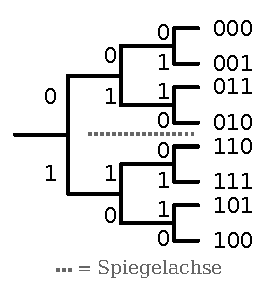
\includegraphics[width=0.8\textwidth]{img/gray_tree.pdf}
		\caption*{Konstruktion eines Gray-Codes mit Baum. Damit sich nur je ein Bit verändert, muss die Beschriftung symmetrisch sein.}
	\end{subfigure}
	\hspace{.07\textwidth}
	\begin{subfigure}{.45\textwidth}
		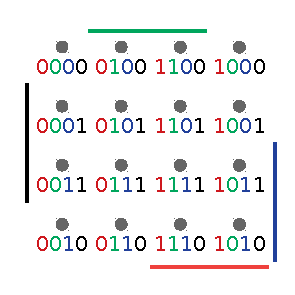
\includegraphics[width=0.8\textwidth]{img/gray_16qam.pdf}
		\caption*{Gray-Labelling einer 16-QAM. Beschriftung mit Variablen wie bei Karnaugh-Diagramm und Wert $n$-ter Variable der $n$-ten Stelle zuordnen.}
	\end{subfigure}
\end{figure}

\section*{Puls-Amplituden Modulation (PAM)}
\begin{figure}[H]
	\begin{subfigure}{0.54\textwidth}
		\[
			a_{k} \in \{-(M - 1) + 2l ~ | ~ l = 0, \ldots, M-1\}
		\]

		Für Normierung $P_S = E \left[|\tilde{a_k}|^2 \right] \overset{!}{=} 1$ wähle
		\[
			\tilde a_k = \mathrm{norm} \cdot a_k \quad \text{mit} \quad \mathrm{norm} = \frac{1}{\sqrt{\frac{M^2 - 1}{3}}}
		\]
	\end{subfigure}
	\begin{subfigure}{0.45\textwidth}
		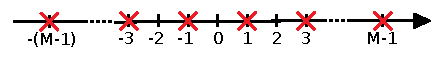
\includegraphics[width=\textwidth]{img/pamconstellation.pdf}
		\caption*{Konstellation der (unnormierten) Symbole $a_k$}
	\end{subfigure}
\end{figure}

\section*{Rauschen und Symbolfehlerwahrscheinlichkeit}
\subsection*{SNR, Signalleistung und Varianz}
Sei $\sigma^2$ \ldots Varianz der Gaußverteilung und $E_s$ \ldots Signalleistung.

\raggedright
Für \textbf{reelles Basisband (AM)} gilt:
\[
	\mathrm{SNR}_s = \frac{P_\mathrm{signal}}{P_\mathrm{noise}} = \frac{E_s}{N_0} = \frac{E_s}{\sigma^2} \quad \overset{E_s = 1}{\implies} \quad \sigma = \frac{1}{\sqrt{\mathrm{SNR}_s}}
\]

\raggedright
Für \textbf{komplexes Basisband (QAM)} teilt sich die Rauschleistung auf beide Dimensionen auf:
\[
	\mathrm{SNR}_s = \frac{P_\mathrm{signal}}{P_\mathrm{noise}} = \frac{E_s}{N_0} = \frac{E_s}{{\color{red} 2} ~ \sigma^2} \quad \overset{E_s = 1}{\implies} \quad \sigma = \frac{1}{\sqrt{2 ~ \mathrm{SNR}_s}}
\]

\raggedright
Die mittlere \textbf{Signalleistung} $P_\mathrm{signal} = E_s$ ist durch den Erwartungswert der Symbolleistung ($x_k \in \mathbb C$ sind die Symbole) gegeben:
\[
	E_s = E[|x_k|^2] = \sum_k P_k |x_k|^2
\]

\subsection*{Allgemein}
\begin{figure}[H]
\centering
\begin{subfigure}{0.54\textwidth}
	\[
		p_n(\xi) = \frac{1}{\sqrt{2 \pi} \sigma} ~ e^{-\frac{1}{2\sigma^2} ~ |\xi|^2} \quad \mathrm{mit} ~ \xi \in \mathbb C ~ \text{oder} ~ \xi \in \mathbb R
	\]
	\[
		P[n \leq c] = \int_{-\infty}^c p_n(\xi) ~ \mathrm d\xi = \mathrm{CDF}\left( \frac{c}{\sigma} \right) = \Phi \left( \frac{c}{\sigma} \right)
	\]
	\[
		P[n > c] = \int_c^\infty p_n(\xi) ~ \mathrm d\xi = \mathrm{CCDF}\left( \frac{c}{\sigma} \right) = Q \left( \frac{c}{\sigma} \right)
	\]
	\[
		\Phi(x) = Q(-x)
	\]
	\[
		Q(x) = 1 - \Phi(x)
	\]
	\[
		\implies \Phi(x) = 1 - \Phi(-x), \quad Q(x) = 1 - Q(-x)
	\]
\end{subfigure}
\begin{subfigure}{0.45\textwidth}
	\caption*{Wahrscheinlichkeitsdichte für $n \sim \mathcal{N}(0, \sigma^2)$}
	\scalebox{0.8}{
	\begin{tikzpicture}
		\begin{axis}[ 
			xlabel = {$\xi$},
			ylabel = {$p_n(\xi)$},
			xmin = -2,
			xmax = 2,
			ymin = -0.2,
			samples = 200
		]

			\addplot[name path=f, green!60!black, mark=none]{1 / (sqrt(0.25 * 2 * pi)) * (e^(-x^2 / (2 * 0.25)))};
			\addplot[name path=axis, black, no markers] coordinates {(-2,0) (2,0)};
			\addplot [mark=none, thick, red!75!black] coordinates {(0.3, -0.05) (0.3, 0.666)};
			\addplot[
				fill=green!60!black, 
				fill opacity=0.2
			]
			fill between[
				of=f and axis,
				soft clip={domain=0.3:2},
			];

			\addplot[
				fill=blue!65!black, 
				fill opacity=0.2
			]
			fill between[
				of=f and axis,
				soft clip={domain=-2:0.3},
			];

		    \node at (axis cs:  0.65, 0.1) {$Q (\frac{c}{\sigma})$};
		    \node at (axis cs:  -0.65, 0.1) {$\Phi(\frac{c}{\sigma})$};
   		    \node at (axis cs:  0.3, -0.1) {\footnotesize{\textit{\color{red!75!black} c}}};
		\end{axis}
	\end{tikzpicture}}
\end{subfigure}
\end{figure}

\subsection*{Für verschiedene Modulationsarten}
Mit Basisbandrauschleistung $N_0 = 2 \sigma_n^2$ ergibt sich Basisband-SNR zu $\mathrm{SNR}_s = \frac{E_s}{N_0}$.

\begin{center}
	\begin{tabular}{r | c c}
		& SER, $P_{s, \mathrm{err}}$ & BER, $P_{b, \mathrm{err}}$, * \\ \hline \\[-1.0em]
		BPSK & $Q \left( \sqrt{2 ~ \mathrm{SNR}_s} \right)$ & $Q \left( \sqrt{2 ~ \mathrm{SNR}_b} \right)$ \\
		QPSK & $\sim 2 ~ Q \left( \sqrt{\mathrm{SNR}_s} \right)$  & $Q \left( \sqrt{2 ~ \mathrm{SNR}_b} \right)$ \\
		M-PSK & $\sim 2 ~ Q \left( \sqrt{2 ~ \mathrm{SNR}_s} ~ \sin(\pi / M) \right)$ & $\sim \frac{2}{\ld(M)} ~ Q \left( \sqrt{2 ~ \mathrm{SNR}_b ~ \ld(M)} ~ \sin(\pi / M) \right)$ \\
		M-PAM & $2 ~ \left( 1 - \frac{1}{M} \right) ~ Q \left(\sqrt{\frac{6}{M^2 - 1} ~ \mathrm{SNR}_s} \right)$ & $~\sim \frac{2}{\ld(M)} ~ \left( 1 - \frac{1}{M} \right) ~ Q \left(\sqrt{\frac{6 ~ \ld(M)}{M^2 - 1} ~ \mathrm{SNR}_b} \right)$ \\
		M-QAM & $\sim 4 ~ Q \left( \sqrt{\frac{3 ~ \mathrm{SNR}_s}{M - 1}} \right)$ & $\sim \frac{4}{\ld(M)} ~ Q \left( \sqrt{\frac{3 ~ \mathrm{SNR}_b ~ \ld(M)}{M - 1}} \right)$
	\end{tabular}
\end{center}

\vspace{5pt}

* Für Coderate $R_c = 1$ (keine Redundanzcodierung) folgt $\mathrm{SNR}_b = \frac{\mathrm{SNR}_s}{M_b} = \frac{\mathrm{SNR}_s}{\ld(M)}$.

Näherung für hohes SNR und Gray-Labeling:
\[
	P_{s, \mathrm{err}} = M_b ~ P_{b, \mathrm{err}}
\]

\section*{QAM}
Möchte Basisbandsignal $z(t) \in \mathbb C$ zu Bandpasssignal $u(t)$ mit Trägerfrequenz $f_0$, $\omega_0 = 2 \pi f_0$ modulieren.

\raggedright
Komplexe Darstellung (Fouriertransformation mit $\Re(z) = \frac{1}{2} (z + z^*)$):
\[
	u(t) = \Re \left \{ x(t) ~ e^{j \omega_0 t} \right \} \ftransform U(f) = \frac{1}{2} ~ \left( X(f - f_0) + X(f + f_0) \right)
\]

\raggedright
Reelle Darstellung:
\[
	u(t) = \Re \{ x(t) \} ~ \cos(\omega_0 t) - \Im \{ x(t) \} ~ \sin(\omega_0 t) \ftransform U(f) = \frac{1}{2} ~ \left( X(f - f_0) + X(f + f_0) \right)
\]

\subsection*{Einseitenband-AM und Hilbertfilter}
Idee: Ein analytisches Signal enthält keine negativen Frequenzen. Aus einem reellen Signal $x(t) \in \mathbb R$ kann ein analytisches Signal $z(t) \in \mathbb C$ ohne Informationsverlust erzeugt werden durch Filterung mit $F(f) = 1 + \sgn(f)$:
\[
	Z(f) = X(f) ~ F(f) = X(f) ~ (1 + \sgn(f)) = X(f) + X(f) ~ \sgn(f)
\]

\raggedright
Mit $\sgn(f) ~~ \Laplace ~~ \frac{j}{\pi t}$ folgt Basisbandsignal für \textbf{upper sideband (USB)}-Modulation:
\[
	z_{\mathrm{USB}}(t) = x(t) + j \left(x(t) * \frac{1}{\pi t} \right)
\]

\raggedright
Analog folgt durch Filterung mit $F(f) = 1 - \sgn(f)$ für \textbf{lower sideband (LSB)}-Modulation:
\[
	z_{\mathrm{LSB}}(t) = x(t) - j \left(x(t) * \frac{1}{\pi t} \right)
\]

$\implies$ $z_{\mathrm{USB}}(t)$ bzw. $z_{\mathrm{LSB}}(t)$ dann einer QAM zuführen!

Das Filter
\[
	g(t) = \frac{1}{\pi t}
\]
wird \textbf{Hilbertfilter} genannt.

\subsection*{Digitale QAM}
Der \textit{\textbf{constellation mapper}} ordnet den Symbolen $M$ verschiedene I/Q-Werte (Konstellationen) zu. Pro Symbol werden also
\[
	M_b = \ld M ~ \left[ \frac{\mathrm{bit}}{\mathrm{symbol}} \right]
\]

Bits übertragen. Mit einer \textbf{Symbolrate} (= Schrittgeschwindigkeit) $R_s ~ \left[\frac{\mathrm{symbol}}{s} = \mathrm{Baud}\right]$ ergibt sich die \textbf{Bitrate} $R_b$ zu
\[
	R_b = M_b ~ R_s \quad \left[ \frac{\mathrm{bit}}{s} \right]
\]

\section*{Sender- / Empfängerunzulänglichkeiten}
\subsection*{Rauschen im Sender}
TX-Rauschen wird durch den EVM-Wert (Error Vector Magnitude) angegeben. Am Senderausgang gilt:
\[
	\mathrm{EVM} = \frac{1}{\mathrm{SNR}} \quad \Leftrightarrow \quad \mathrm{EVM}|_{\mathrm{dB}} = - \mathrm{SNR}|_{\mathrm{dB}}
\]

\subsection*{Phasenoffset}
Ein geschätztes Phasenoffset von $\hat \varphi$ kann durch Multiplikation der Empfangssymbole mit $e^{-j \varphi}$ korrigiert werden.

\subsection*{Frequenzoffset}
Für jedes Symbol steigt der Phasenoffset um
\[
	\varphi_{\mathrm{inc}} = 2 \pi f_{\mathrm{off}} ~ T_s
\]

\subsection*{IQ-Imbalance}
DC-Offset des Q-Kanals um $d_{\mathrm{imb}}$, Phasenoffset des Q-Kanals um $\varphi_{\mathrm{imb}}$, Amplitudenoffset des Q-Kanals um $a_{\mathrm{imb}}$. Aus idealem Symbol $s \rightarrow \mathbf s = (\Re(s) ~~ \Im(s))^T$ wird $s_{\mathrm{imb}} \rightarrow \mathbf s_{\mathrm{imb}} = (\Re(s_{\mathrm{imb}}) ~~ \Im(s_{\mathrm{imb}}))^T$:
\[
	\mathbf s_{\mathrm{imb}} = \begin{pmatrix}
		1 & -a_\mathrm{imb} ~ \sin(\varphi_\mathrm{imb}) \\
		0 & ~~ a_\mathrm{imb} ~ \cos(\varphi_\mathrm{imb})
	\end{pmatrix} ~ \mathbf s + \begin{pmatrix}
		0 \\
		d_\mathrm{imb}
	\end{pmatrix}
\]

Schätzung der IQ-Imbalance durch Pilotsymbole, Kompensation durch Inversion der obigen Gleichung.

\section*{OFDM und FFT / iFFT}
\begin{itemize}
\item Ein \textbf{OFDM-Symbol} besteht üblicherweise aus \textbf{$N_{\mathrm{sub}}$ QAM-Symbolen} auf den jeweiligen Unterträgern
\item OFDM-Symbol-\textbf{Schrittgeschwindigkeit} $R_s = \frac{1}{T_s}$
\item \textbf{Abtastrate} $R_{\mathrm{samp}} = \frac{1}{T_{\mathrm{samp}}} = N_{\mathrm{sub}} ~ R_s = \frac{T_s}{N_{\mathrm{sub}}}$
\item OFDM-Symbol-Index $k$ mit $t = k ~ T_s$
\item Abtastwertindex $m$ (``schnelle Zeit'') mit $t = m ~ T_{\mathrm{samp}}$, d.h. $N_{\mathrm{sub}}$ Abtastwerte pro OFDM-Symbol
\item Moduliere unterträger mit $M_b = \ld(M)$ bits pro Symbol
\end{itemize}


Dann gilt für Bitrate $R_b$, Unterträgerabstand $\Delta f$ und gesamte Bandbreite $B$:
\[
	R_b = M_b ~ N_{\mathrm{sub}} ~ R_s
\]
\[
	B = R_{\mathrm{samp}} = N_{\mathrm{sub}} ~ R_s
\]
\[
	\Delta f = R_s
\]

\tikzstyle{transform} = [rectangle, thick, draw, node distance=20pt and 20pt, text width=65pt, text centered, minimum height=40pt]
\tikzstyle{converter} = [rectangle, thick, draw, node distance=20pt and 20pt, text width=30pt, text centered, minimum height=40pt, minimum width=40pt]
\tikzstyle{channel} = [rectangle, thick, draw, node distance=20pt and 20pt, text width=65pt, text centered, rounded corners=3pt, minimum height=40pt, fill=green!20]
\tikzstyle{dataflow} = [draw, -latex, thick]

\begin{figure}[H]
	\centering
	\begin{tikzpicture}
		\node (input) {$\mathbf s_k$};
		\node [transform, right = 0.3cm of input] (fh) {\huge $\mathbf F^H$};
		\node [converter, right = of fh] (da) {D/A};
		\node [channel, right = 2cm of da] (modulation) {Modulation auf Kanal};
		\node [converter, right = of modulation] (ad) {A/D};
		\node [transform, right = of ad] (f) {\huge $\mathbf F$};
		\node [right = 0.3cm of f] (output) {$\hat{\mathbf s}_k$};

		\path [dataflow] (input) -- (fh);
		\path [dataflow] (fh) -- node[midway,above] {$\mathbf x_k$} (da);
		\draw (da.east) to[lowpass, l=RLP] (modulation.west);
		\path [dataflow] (modulation) -- (ad);
		\path [dataflow] (ad) -- node[midway,above] {$\hat{\mathbf x}_k$} (f);
		\path [dataflow] (f) -- (output);
	\end{tikzpicture}
	\caption*{OFDM-Sender und -Empfänger unter der Annahme, dass D/A bzw. A/D-Wandler direkt $N_{\mathrm{sub}}$ Symbole serialisieren / parallelisieren}
\end{figure}

Habe für $k = \left \lfloor \frac{m}{N_{\mathrm{sub}}} \right \rfloor$-ten Zeitschritt
\begin{center}
\begin{tabular}{r p{9cm}}
	$m = k ~ N_{\mathrm{sub}}, \ldots, (k + 1) ~ N_{\mathrm{sub}} - 1$ & Schnelle Zeit mit $N_{\mathrm{sub}}$ Zeitindizes pro $k$ \\
	$s_m \in \mathbb C$ & $N_\mathrm{sub}$ zu sendende Symbole \\
	$\mathbf s_k = (s_{k N_\mathrm{sub}}, \ldots, s_{(k + 1) N_\mathrm{sub} - 1}) \in \mathbb C^{N_\mathrm{sub} \times 1}$ & Frequenzbereichsvektor mit $N_{\mathrm{sub}}$ zu sendenden Symbolen (parallelisiert aus $s_m$) \\
	$\mathbf x_k \in \mathbb C^{N_\mathrm{sub} \times 1}$ & Zeitbereichsvektor mit $N_{\mathrm{sub}}$ zu sendenden Abtastwerden \\
	$x_m = \mathbf x_k[m \mod N_{\mathrm{sub}}] \in \mathbb C$ & Zu sendende Abtastwerte (serialisiert aus $\mathbf x_k$) \\
\end{tabular}
\end{center}

Es gilt (da $\mathbf F$ unitär):
\[
	\mathbf x_k = \mathbf F^H ~ \mathbf s_k \quad \Leftrightarrow \quad \mathbf s_k = \mathbf F ~ \mathbf x_k, \qquad \text{wobei} ~ \mathbf F^{-1} = \mathbf F^H = \mathbf F^*
\]

Mit $W := e^{\frac{2 \pi}{N_{\mathrm{sub}}}}$:
\[
	\mathbf F^H = \frac{1}{\sqrt{N_\mathrm{sub}}} \begin{pmatrix}
		W^0 & W^0 & W^0 & \ldots & W^0 \\
		W^0 & W^1 & W^2 & \ldots & W^{N_\mathrm{sub} - 1} \\
		W^0 & W^2 & W^4 & \ldots & W^{2 (N_\mathrm{sub} - 1)} \\
		\vdots & & & \ddots & \vdots \\
		W^0 & W^{N_\mathrm{sub} - 1} & W^{2(N_\mathrm{sub} - 1)} & \ldots & W^{(N_\mathrm{sub} - 1)^2}
	\end{pmatrix} \in \mathbb C^{N_\mathrm{sub} \times N_\mathrm{sub}}
\]

\[
	\mathbf F = \frac{1}{\sqrt{N_\mathrm{sub}}} \begin{pmatrix}
		W^0 & W^0 & W^0 & \ldots & W^0 \\
		W^0 & W^{-1} & W^{-2} & \ldots & W^{-(N_\mathrm{sub} - 1)} \\
		W^0 & W^{-2} & W^{-4} & \ldots & W^{-2 (N_\mathrm{sub} - 1)} \\
		\vdots & & & \ddots & \vdots \\
		W^0 & W^{-(N_\mathrm{sub} - 1)} & W^{-2(N_\mathrm{sub} - 1)} & \ldots & W^{-(N_\mathrm{sub} - 1)^2}
	\end{pmatrix} \in \mathbb C^{N_\mathrm{sub} \times N_\mathrm{sub}}
\]

\section*{Mathe-Formelsammlung}
\subsection*{Additionstheoreme}
\begin{multicols}{2}
\[ \sin(\alpha) ~ \cos(\beta) = \frac{1}{2} (\sin(\alpha - \beta) + \sin(\alpha + \beta)) \]
\[ \cos(\alpha) ~ \cos(\beta) = \frac{1}{2} (\cos(\alpha - \beta) + \cos(\alpha + \beta)) \]
\[ \sin(\alpha) ~ \sin(\beta) = \frac{1}{2} (\cos(\alpha - \beta) - \cos(\alpha + \beta)) \]
\vspace{0.5pt}
\[ \sin(\alpha + \beta) = \sin(\alpha) ~ \cos(\beta) + \cos(\alpha) ~ \sin(\beta) \]
\[ \sin(\alpha - \beta) = \sin(\alpha) ~ \cos(\beta) - \cos(\alpha) ~ \sin(\beta) \]
\[ \cos(\alpha + \beta) = \cos(\alpha) ~ \cos(\beta) - \sin(\alpha) ~ \sin(\beta) \]
\[ \cos(\alpha - \beta) = \cos(\alpha) ~ \cos(\beta) + \sin(\alpha) ~ \sin(\beta) \]
\end{multicols}
\vspace{0.5pt}
\[ \sin^2(\alpha) + \cos^2(\alpha) = 1 \]
\[ \sin^2(\alpha) - \cos^2(\alpha) = -\cos(2\alpha) \]
\[ \cos^2(\alpha) - \sin^2(\alpha) = \cos(2\alpha) \]
\[ \cos(x)^2 = \frac{1}{2} \left(1 + \cos(2x) \right) \qquad \sin(x)^2 = \frac{1}{2} \left(1 - \cos(2x) \right) \]

\subsubsection*{Wichtige Eigenschaften der Fouriertransformation}
\begin{multicols}{2}
	\fancyformula{Spiegelung}{\[ x(-t) \ftransform X(-\omega) \]}
	\fancyformula{Konjugiert komplex}{\[ x^*(t) \ftransform X^*(-\omega)\]}
	\fancyformula{Verschiebung}{
		\begin{align*}
			x(t - t_0) & \ftransform e^{-j \omega t_0} ~ X(\omega) \\
			e^{j \omega_0 t} ~ x(t) & \ftransform X(\omega - \omega_0)
		\end{align*}
	}	
	\fancyformula{Anfangswert}{
		\[ X(0) = \int_{-\infty}^{\infty} x(t) ~ \mathrm dt \qquad x(0) = \int_{-\infty}^{\infty} X(\omega) ~ \frac{\mathrm d\omega}{2 \pi} \]	
	}
\end{multicols}


\subsubsection*{Wichtige Fouriertransformationen}
Sei Definition der Rechteckfunktion:
\[
	\rect(t) = \begin{cases}
		1 & \text{für } |t| < 1\\
		0 & \text{für } |t| > 1\\
	\end{cases}
\]

Seien $t_0 > 0$, $\omega_0 > 0$:
\begin{multicols}{2}
	\[ \rect \left(\frac{t}{t_0} \right) \ftransform 2 t_0 ~ \sinc(t_0 ~ \omega) \]
	\[ \frac{\omega_0}{\pi} ~ \sinc(\omega_0 t) \ftransform \rect \left( \frac{\omega}{\omega_0} \right) \]
	\[ \cos(\omega_0 t - \varphi) \ftransform \pi ~ [\delta(\omega - \omega_0) ~ e^{-j \varphi} + \delta(\omega + \omega_0) ~ e^{j \varphi}] \]
	\[ \sin(\omega_0 t - \varphi) \ftransform \frac{\pi}{j} ~ [\delta(\omega - \omega_0) ~ e^{-j \varphi} - \delta(\omega + \omega_0) ~ e^{j \varphi}] \]
	\[ x(t) ~ \cos(\omega_0 t - \varphi) \ftransform \frac{1}{2} ~ \left[X(\omega - \omega_0) ~ e^{-j \varphi} + X(\omega + \omega_0) ~ e^{j \varphi} \right]\]
	\[ x(t) ~ \sin(\omega_0 t - \varphi) \ftransform \frac{1}{2j} ~ \left[X(\omega - \omega_0) ~ e^{-j \varphi} - X(\omega + \omega_0) ~ e^{j \varphi} \right]\]
	\[ \frac{1}{\pi t} \ftransform - j \sgn(\omega)\]
\end{multicols}

\subsubsection*{Rechteckimpulsformer}
\begin{figure}[H]
	\begin{subfigure}{0.45\textwidth}
		\caption*{Rechteckimpuls $g(t)$ im Zeitbereich}
		\centering
		\scalebox{0.8}{
		\begin{tikzpicture}
			\begin{axis}[
				axis lines=center, 
				xlabel = {$t$},
				ylabel = {$g(t)$},
				xticklabels = {$-T_s / 2$, $T_s / 2$},
				xtick = {-0.5, 0.5},
				xmin = -2,
				xmax = 2,
				ymin = -0.3,
				ymax = 1.2,
				samples = 200
			]
				\addplot+[blue!60!black, thick, no marks, const plot] coordinates {(-2,0)(-1,0)(-0.5,1)(0,1)(0.5,0)(2,0)};
			\end{axis}
		\end{tikzpicture}}
		\[ g(t) = \rect \left( \frac{t}{T_s / 2} \right) \]
	\end{subfigure}
	\begin{subfigure}{0.1\textwidth}
		\centering
		\huge
		\[\ftransform\]
	\end{subfigure}
	\begin{subfigure}{0.45\textwidth}
		\caption*{$\sinc$-Frequenzspektrum G(f)}
		\centering
		\scalebox{0.8}{
		\begin{tikzpicture}
			\begin{axis}[ 
				axis lines = center,
				xlabel = {$f$},
				ylabel = {$G(f)$},
				xticklabels = {$-2 R_s$, $-R_s$, $R_s$, $2 R_s$},
				xtick = {-2, -1, 1, 2},
				yticklabels = {$T_s$},
				ytick = {1},
				xmin = -3.2,
				xmax = 3.2,
				ymin = -0.3,
				ymax = 1.2,
				samples = 200
			]
				\addplot[green!60!black, thick, no marks]{sin(pi*deg(x))/(pi*x)};
			\end{axis}
		\end{tikzpicture}}
		\[ G(f) = T_s ~ \sinc \left(\pi T_s f \right) = \frac{1}{R_s} ~ \sinc \left(\frac{\pi f}{R_s} \right) \]
	\end{subfigure}
\end{figure}

\subsubsection*{$\sin(x) / x$-Impulsformung}
\begin{figure}[H]
	\begin{subfigure}{0.45\textwidth}
		\caption*{$\sin(x) / x$ im Zeitbereich}
		\centering
		\scalebox{0.8}{
			\begin{tikzpicture}
			\begin{axis}[
				axis lines = center, 
				xlabel = {$t$},
				ylabel = {$g(t)$},
				xticklabels = {$-T_s$, $T_s$},
				xtick = {-1, 1},
				xmin = -3.2,
				xmax = 3.2,
				ymin = -0.3,
				ymax = 1.2,
				samples = 200
			]
				\addplot[blue!60!black, thick, no marks]{sin(pi*deg(x))/(pi*x)};			
			\end{axis}
			\end{tikzpicture}}
		\[ g(t) = \sinc\left(\frac{\pi t}{T_{S}}\right) \]
	\end{subfigure}
	\begin{subfigure}{0.1\textwidth}
		\centering
		\huge
		\[\ftransform\]
	\end{subfigure}
	\begin{subfigure}{0.45\textwidth}
		\caption*{$\rect$-Frequenzspektrum G(f)}
		\centering
		\scalebox{0.8}{
			\begin{tikzpicture}
				\begin{axis}[ 
					axis lines = center,
					xlabel = {$f$},
					ylabel = {$G(f)$},
					xticklabels = {$-R_s / 2$, $R_s / 2$},
					xtick = {-0.5, 0.5},
					yticklabels = {$T_s$},
					ytick = {1},
					xmin = -2,
					xmax = 2,
					ymin = -0.3,
					ymax = 1.2,
					samples = 200
				]
				\addplot[green!60!black, thick, no marks, const plot] coordinates {(-2,0)(-1,0)(-0.5,1)(0,1)(0.5,0)(2,0)};
			\end{axis}
			\end{tikzpicture}}
		\[
		G(f) = T_s ~ \rect(2 T_s ~ f) = \frac{1}{R_s} ~ \rect \left(\frac{f}{R_s / 2} \right) \]
	\end{subfigure}
\end{figure}

\end{document}